\documentclass[tikz,border=2pt]{standalone}
\usepackage{tikz}

\begin{document}
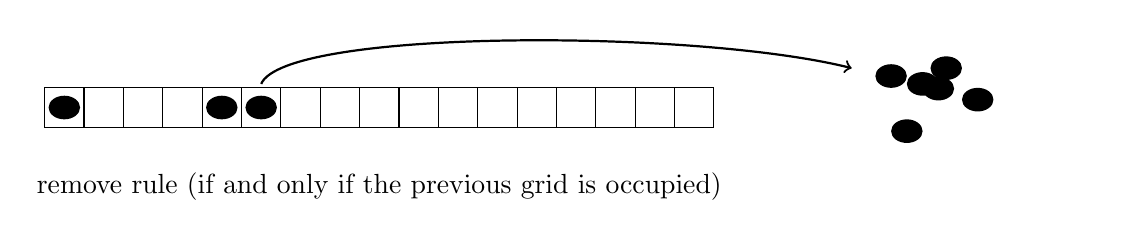
\begin{tikzpicture}[scale=1.0]

\def\y{0}
\node at (4, \y-1) {remove rule (if and only if the previous grid is occupied)};
\foreach \x in {0,...,16}
	\draw (0.5*\x-0.25, 0.5*\y-0.25) rectangle (0.5*\x+0.25, 0.5*\y+0.25);
\fill (0, 0)  ellipse (0.2 and 0.15);
\fill (2, 0)  ellipse (0.2 and 0.15);
\fill (2.5, 0)  ellipse (0.2 and 0.15);
\def\dx{11}
\foreach \a/\b in {-0.1/0.3, 0.2/0.5, -0.5/0.4, 0.1/0.24, 0.6/0.1, -0.3/-0.3}
	\fill (\dx+\a, \y+\b)  ellipse (0.2 and 0.15);
\node at (13, -1) {};
\draw[->,thick] (2.5, \y+0.3) .. controls (2.8, \y+1) and (8.0, \y+1) .. (10, 0.5);

\end{tikzpicture}
\end{document}
